\documentclass[onecolumn,11pts]{IEEEtran}
\usepackage[utf8]{inputenc}
\usepackage{listings}
\usepackage{xcolor}
\usepackage{url}
\usepackage{hyperref}
\usepackage{graphicx}
\usepackage{anysize}
\usepackage[spanish]{babel} 
\usepackage[utf8]{inputenc} 
\usepackage{multirow}
\marginsize{3.5cm}{2.5cm}{3cm}{3cm} 
\hypersetup{
  colorlinks=false,       % false: boxed links; true: colored links
  pdfborder={0 0 0}       % remove ugly border from links
}


\markboth{Redes de Datos}%
{Informe}
\date{November 2016}

\begin{document}

\begin{titlepage}

\begin{center}
\vspace*{-1in}
\begin{figure}[htb]
\begin{center}

\includegraphics[scale=0.4]{logo_udp}
\end{center}
\end{figure}
Facultad de Ingeniería y Ciencias\\Escuela de Informática y Telecomunicaciones\\
\vspace*{0.15in}
\vspace*{1in}

\begin{LARGE}
\textbf{Laboratorio N4: Redes de Datos\\
Comprobación del funcionamiento del algoritmo STP e\\
implementación de VLAN} \\
\end{LARGE}
\vspace*{1in}
\begin{large}
Profesor: José Pérez \\Ayudante: Alexis Inzunza \\ Fecha: 26-05-2017
\end{large}
\vspace*{0.3in}
\vspace*{1in}
\begin{large}
\begin{flushright}

Integrantes: \\
Benjamín Alvarez \\ Nicolás Reyes \\ 
\end{flushright}
\end{large}
\end{center}
\end{titlepage}


\tableofcontents % indice de contenidos

\cleardoublepage

\cleardoublepage
\listoffigures
\title{Actividades de Laboratorio}

\maketitle

\section{Actividad: Configuración de STP, topología con bucles y priorización de STP}
    Para la primera actividad realizamos una topología en packet tracer para estudiar cómo funciona spanning tree protocol (STP), para esto utilizamos 3 switch 2950  conectados entre si y 3 computadores, cada computador conectado a un switch diferente. Como se muestra en la siguiente imagen:
    
   \begin{figure}[h!]
\centering
 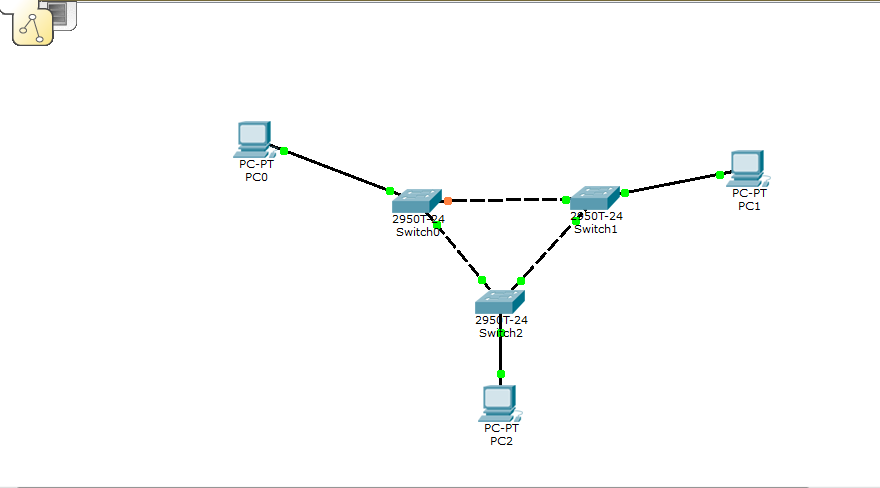
\includegraphics[scale=0.5]{topo1}
\caption{Topología ejercicio STP}
\label{fig:topo1}
\end{figure}

Como no hemos asignado ninguna VLAN trabajaremos con la 1 (que viene por default) y como observamos en la imagen STP actúa inmediatamente cuando se presenta un bucle . para observar cómo funciona STP tendremos que desactivar STP para la VLAN 1. Esto se puede realizar con los siguientes comandos:(Esto lo  realizamos para los tres switch)\\

\begin{figure}[h!]
\centering
 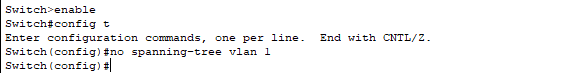
\includegraphics[scale=0.8]{comand-nostp}
\caption{Comandos para quitar STP de los Switches}
\label{fig:comand-nostp}
\end{figure}

Usando estos comandos en cada Switch tenemos como resultado un cambio en sus puertos, ya que ahora todos los puertos están encendidos, como se muestra en la Figura 3.\\También si hacemos ping desde cualquier PC a otro vamos a ver como el paquete nunca llega a su destino ya que se crea un bucle donde el paquete gira por los Switches.
\begin{figure}[h!]
\centering
 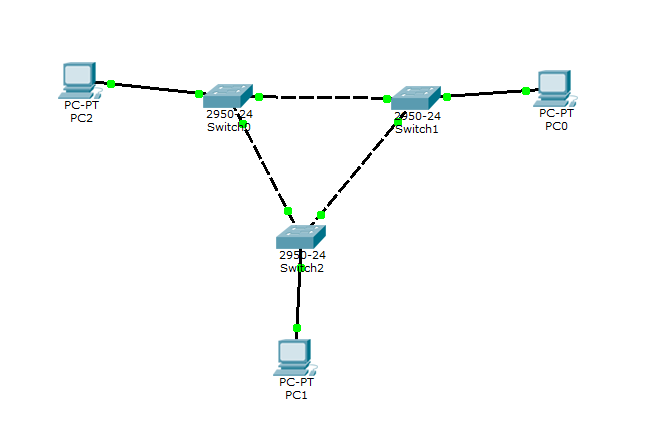
\includegraphics[scale=0.5]{stpapagado}
\caption{Topología con STP desactivado}
\label{fig:stpapagado}
\end{figure}

\newpage
Ahora para volver a la topología con STP debemos activarlo en todos los Switches usando el siguiente comando:

\begin{figure}[h!]
\centering
 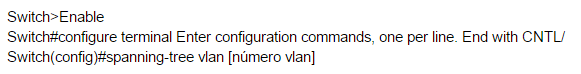
\includegraphics[scale=0.8]{com-stpon}
\caption{Comandos para volver a activar STP en los Switches}
\label{fig:com-stpon}
\end{figure}
Luego de esto se nos pide en la actividad dos modificar la prioridad de dos de los switches, tomando como primario el switch 1 y como secundario cualquiera de los otros dos switches.\\
Para hacer esto nuevamente se usarán dos comandos para poner los routers como primario y secundario.\\
Para primario se usará este comando:
\begin{figure}[h!]
\centering
 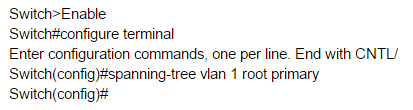
\includegraphics[scale=0.8]{stpprimary}
\caption{Comandos para primario}
\label{fig:stpprimary}
\end{figure}
Y para secundario se usará el siguiente:
\begin{figure}[h!]
\centering
 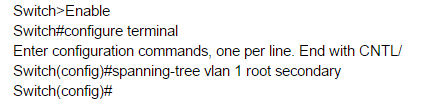
\includegraphics[scale=0.8]{stpsecondary}
\caption{Comandos para secundario}
\label{fig:stpsecondary}
\end{figure}

Como lo aprendimos en clases el switch con la menor prioridad  va a ser el root bridge y existe un comando para cambiar las prioridades en lo switch que es el siguiente:

\begin{figure}[h!]
\centering
 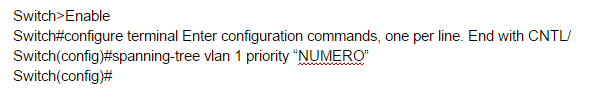
\includegraphics[scale=0.8]{stpprority}
\caption{Comandos para cambiar prioridad}
\label{fig:stpprority}
\end{figure}

La prioridad tiene un rango asignable de [0-61440] y este número se va incrementando en múltiplos de 4096.
\newpage
\section{Actividad: Configuración de VLAN}

En esta actividad se nos pide construir la siguiente topología:

\begin{figure}[h!]
\centering
 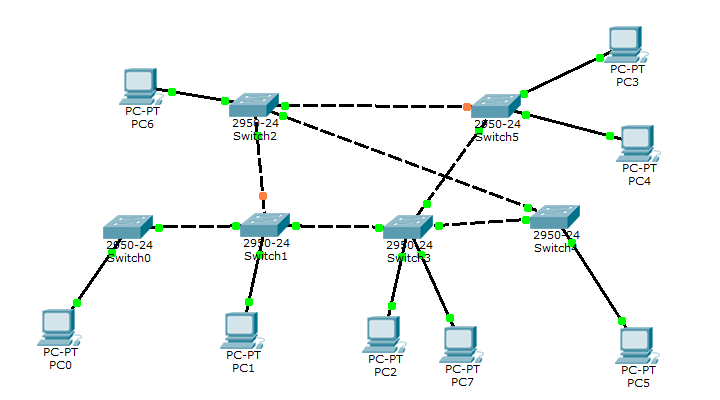
\includegraphics[scale=0.5]{ss1}
\caption{Topología VLAN}
\label{fig:ss1}
\end{figure}
Y tambien usar la siguiente tabla para configurar las VLAN en los switches dependiendo de cada PC:
\begin{figure}[h!]
\centering
 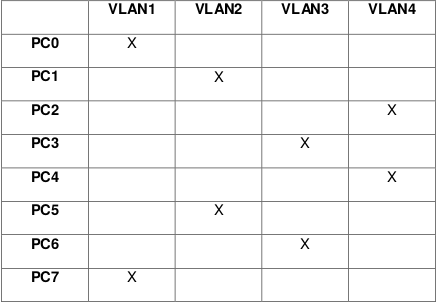
\includegraphics[scale=0.8]{tablavlan}
\caption{Tabla de VLAN}
\label{fig:tablavlan}
\end{figure}
\newpage
Empezamos asignando las VLAN de la tabla a los switch correspondiente con los siguientes comandos:
\begin{figure}[h!]
\centering
 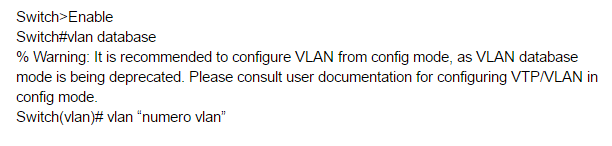
\includegraphics[scale=0.8]{agvlan}
\caption{Comando para agregar VLAN a un Switch}
\label{fig:tablavlan}
\end{figure}

Luego asignamos los puertos trunk y access según corresponda. En este caso los puertos access son los de switches conectados a PC's y los que estan entre switches serán los puertos trunk.\\
Los comandos para asignar el modo access son:
\begin{figure}[h!]
\centering
 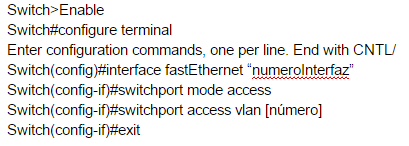
\includegraphics[scale=0.8]{access}
\caption{Comandos para mode access}
\label{fig:acess}
\end{figure}

\\Y para el modo Trunk son:
\begin{figure}[h!]
\centering
 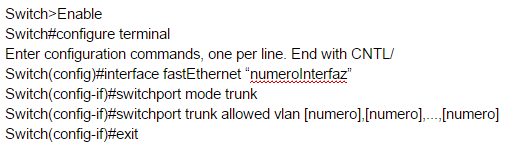
\includegraphics[scale=0.8]{trunk}
\caption{Comandos para mode trunk}
\label{fig:trunk}
\end{figure}
\\Después de haber configurado cada puerto ahora tendremos que ponerle IP's a los PC's. Para eso usaremos el segmento 10.0.0.1/24. El PC 0 tiene debe tener IP 10.0.0.8 para esta actividad, mientras que los otros pueden tener cualquier IP mientras esten en el segmento.\\
Las IP's que tendrán los PC's son las siguientes:

\begin{figure}[h!]
\centering
 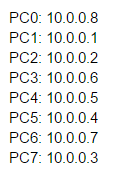
\includegraphics[scale=0.8]{ipspc}
\caption{Ip's que tendrán los PC's}
\label{fig:ipspc}
\end{figure}
\newpage
Cuando terminamos esta configuración nuestra topología esta lista y para verificar su correcto funcionamiento hacemos ping a todos lados y así verificamos que nuestra topología está correctamente configurada.


\newpage
\section{Preguntas propuestas}
\subsection{Actividad 1}
\begin{enumerate}
    \item ¿Qué camino realizara un paquete que para llegar desde el switch 0 hasta el switch 2?\\
R: Primero aclarar que en cualquier caso donde en los switches no esté presente el protocolo STP se creará un bucle con el mensaje a mandar, por lo tanto este nunca llega a su destino, ya que solo gira a través de las switches.
Con el protocolo STP activado en todos los switchs y tomando como referencia el siguiente ejemplo de la FIGURAx, tenemos que realiza desde el switch 0 al switch 2 será el siguiente: Desde el switch 0 se mandará el paquete a los Switchs 1 y 2, luego este se mandará estos lo mandarán a sus respectivos PC’s para verificar que el paquete llegue a su destino, exceptuando el switch 2 que mandará el paquete al Switch 1, aunque sin éxito, ya que el puerto fa0/3 está apagado por el protocolo STP. Después de eso el paquete se devuelve desde el Switch 2 a el 0 para confirmar que llegó correctamente.\\

    \item ¿Qué camino realizara un paquete que para llegar desde el switch 2 hasta el switch1?\\
R: Desde el Switch 2 se mandará el paquete a el Switch 0 y al 1, pero fallando con el Switch 1 ya que su puerto lo tiene apagado. Luego el Switch 0 mandará el paquete a su respectivo PC y a el Switch 1. Ya que el PC que se encuentra en el Switch 0 no es el que debe recibir el paquete este lo rechaza y el Switch 1 manda el paquete a su PC y comprueba que sea el que se busca. Una vez comprobado el paquete se devuelve desde el Switch 1 al Switch 0 y luego al 2 para que este sepa que el paquete llegó correctamente.\\

    \item ¿Qué camino realizara un paquete que para llegar desde el switch 2 hasta el switch0?\\
R: Poniendo el Switch 1 como primario el Switch 2 como secundario nos quedará como en la siguiente FIGURA.
El paquete parte desde el Switch 2, y lo manda a el Switch 1. Una vez ahí, el Switch 1, manda el paquete a su respectivo PC y al Switch 0. Como el paquete va para el Switch 0 el Switch 1 lo rechaza y luego se devuelve por el mismo camino hacia el Switch 2 para confirmar que el paquete llega correctamente.\\
    \item ¿Qué camino realizara un paquete que para llegar desde el switch 1 hasta el switch0?\\
R: En este caso el paquete se manda desde el Switch 1 a los Switch 0 y 2. Una vez recibidos el Switch 0 confirma que a él se le había mandado el paquete, mientras que el Switch 2 manda el paquete a el Switch 0 y a su PC, sin tener un bueno resultado en ninguno de los dos, ya que el paquete no iba al PC 2 y ya que el protocolo STP está activado en la topología el paquete nunca llega a su destino, el Switch 0. Ahora el paquete se devolverá al Switch 1 para comprobar que el paquete llegó correctamente a su destino.

\end{enumerate}
\newpage
\subsection{Actividad 2}
\begin{enumerate}
    \item ¿Cuál es la diferencia del modo Access y el modo Trunk en un switch?\\
R: La principal diferencia se encuentra en la utilidad que tienen esto puertos. En el caso de el puerto Access solo pueden transportar tráfico de una sola VLAN  y generalmente va conectada desde un Switch a equipos finales, aunque igualmente se puede entre Switches, pero no es muy recomendable. Mientras que el puerto Trunk es principalmente para la conexión entre Switches y además puede transportar tráfico de múltiples VLAN’s.\\
    \item ¿Qué ocurre si conecto una puerta en modo Trunk a un PC?
R: No debería tener problema, siempre y cuando todos los Switch estén bien configurados, pero sería redundante ya que solo se necesita que llegue una VLAN (la que se esté usando para el PC).\\
    \item ¿Qué ocurre si conecto dos switches, uno en modo access y otro en modo trunk?\\
R: Solo podrián transportar paquetes de la VLAN puesta en el modo Access, siempre y cuando esta se encuentre las VLAN’s configuradas en el Trunk.\\
    \item ¿Qué camino realizara un paquete que para llegar desde el switch 1 hasta el switch 0?\\
    R: El paquete saldrá desde el Switch 1 y se dirigirá hacia el Switch 0 y el 3. El del Switch 0 comprueba si es de la misma VLAN o no y luego lo regresa confirmando si llegó o no. Mientras el otro paquete recorre todas las otras VLAN buscando el PC 0 y confirmando que efectivamente no está en ese sector. 




\end{enumerate}
\newpage
\section{Conclusión}
Con este laboratorio pudimos enternder como funciona el protocolo STP, configurando una topología simple de distinantas formas, cambiando las prioridad e incluso creando un bucle, todo esto con la intención de ver como se transportan los paquetes con este protocolo. También pudimos configurar una topología con VLAN's y vimos lo costoso que puede ser configurar ciertos puertos con trunk o access, pero todo esto tuvo un resultado exitoso al poder comunicar correctamente las VLAN's. También nos dimos cuenta de la importancia de las VLAN's en redes de trabajo, como en la misma universidad, para poder manejar a lo que pueden o no acceder los usuarios.


\clearpage

\begin{thebibliography}{15}

\bibitem{mfp}
  quora,
  \emph{Computer Networking: Is it possible to have a trunk on a switchport connected to a PC (not a switch-to-switch)? If it is possible, does it have the same procedure just like setting trunk between two switches? }
  \url{https://www.quora.com/Computer-Networking-Is-it-possible-to-have-a-trunk-on-a-switchport-connected-to-a-PC-not-a-switch-to-switch-If-it-is-possible-does-it-have-the-same-procedure-just-like-setting-trunk-between-two-switches}
  \bibitem{mfp}
  capa8net,
  \emph{Tipos de puertos Access – Trunk}
  \url{https://capa8net.wordpress.com/2014/02/13/tipos-de-puertos-access-trunk/}

\end{thebibliography}

\end{document}